\documentclass[aspectratio=169, 11pt]{beamer}

% SSS-Rank Minimalist Theme
\usetheme{default}
\useinnertheme{circles}
\setbeamertemplate{navigation symbols}{} % Убиваем уродливые иконки внизу
\setbeamertemplate{footline}[frame number] % Оставляем только номера слайдов

\usepackage{amsmath, amssymb, amsthm}
\usepackage{bm}
\usepackage{booktabs}
\usepackage{graphicx}
\usepackage{xcolor}

% Custom Colors (Cold & Professional)
\definecolor{miptblue}{RGB}{0, 84, 166}
\definecolor{darkgray}{RGB}{50, 50, 50}
\definecolor{accentred}{RGB}{200, 30, 30}

% Theme coloring
\setbeamercolor{title}{fg=miptblue}
\setbeamercolor{frametitle}{fg=miptblue, bg=white}
\setbeamercolor{itemize item}{fg=miptblue}
\setbeamercolor{itemize subitem}{fg=miptblue}
\setbeamercolor{enumerate item}{fg=miptblue}
\setbeamerfont{frametitle}{series=\bfseries}

% Math shortcuts
\newcommand{\norm}[1]{\left\|#1\right\|}
\newcommand{\JF}{J_F}
\newcommand{\JMSA}{J_{\mathrm{MSA}}}
\newcommand{\JFFN}{J_{\mathrm{FFN}}}
\newcommand{\RMS}{\mathrm{RMSNorm}}

\title{\LARGE \textbf{Jacobian Analysis of a Recurrent\\ Transformer Block}}
\author{\vspace{1em} Dmitrii Vasilenko \and Ilia Stepanov \and Vadim Kasiuk \and \\ Gleb Karpeev \and Andrey Grabovoy}
\institute{\vspace{0.5em} \textit{Moscow Institute of Physics and Technology}}
\date{\vspace{1em} \textcolor{miptblue}{\textbf{AINL 2026}}}

\begin{document}

% ---------------------------------------------------------------
\begin{frame}[plain]
    \titlepage
\end{frame}
% ---------------------------------------------------------------
\begin{frame}{Why Study Recurrent Transformers?}
    \begin{columns}
        \begin{column}{0.55\textwidth}
            \textbf{Looped (Recurrent) Architectures:}
            \begin{itemize}
                \item Reuse the same block across iterations.
                \item Parameter-efficient: depth $\neq$ model size.
            \end{itemize}

            \vspace{1em}
            \textbf{Key Question:}\\
            Do repeated applications of $F$ converge stably, or does the gradient explode?
        \end{column}
        \begin{column}{0.45\textwidth}
            \textbf{Iterative Map:}
            \[
                Y^{(t+1)} = F\!\left(Y^{(t)}\right)
            \]
            \[
                F(Y) = \RMS\!\left(Y + \nu\bigl(C + \mathrm{TB}(Y)\bigr)\right)
            \]

            \vspace{1em}
            \small
            $\nu > 0$ — Step size coefficient\\
            $C = Y^{(0)}$ — External context
        \end{column}
    \end{columns}
\end{frame}

% ---------------------------------------------------------------
\begin{frame}{The Role of the Jacobian}
    \textbf{Why Jacobians?}
    \begin{itemize}
        \item Classical tool for local stability analysis.
        \item If $\norm{J_F(Y)}_2 < 1 \Rightarrow$ local contraction $\Rightarrow$ stability.
    \end{itemize}

    \vspace{1.5em}
    \textbf{Prior Work \small{(Tomihari \& Karakida, 2025)}:}
    \begin{itemize}
        \item Analyzed dynamics for \textit{self-attention only} blocks.
    \end{itemize}

    \vspace{1.5em}
    \textbf{Our Contribution:}\\
    We extend this framework to a full Transformer block including MSA, FFN, residual connections, and RMSNorm.
\end{frame}

% ---------------------------------------------------------------
\begin{frame}{Architecture: Post-Norm Transformer Block}
    \textbf{Notation:} State $Y^{(t)} \in \mathbb{R}^{S \times D}$ with sequence length $S$, hidden dimension $D$.

    \vspace{1.5em}
    \textbf{Sub-blocks:}
    \[
        Y' = \RMS\!\left(Y + \mathrm{MSA}(Y)\right)
    \]
    \[
        \mathrm{TB}(Y) = \RMS\!\left(Y' + \mathrm{FFN}(Y')\right)
    \]

    \vspace{1em}
    \textbf{Full Iterative Update:}
    \[
        Y^{(t+1)} = \RMS\!\left(Y^{(t)} + \nu\bigl(C + \mathrm{TB}(Y^{(t)})\bigr)\right)
    \]

    \vspace{1em}
    \small \textcolor{darkgray}{*Row-wise RMSNorm defined as: $\RMS(y) = \mathrm{diag}(\gamma)\,\frac{y}{\|y\|_2}$}
\end{frame}

% ---------------------------------------------------------------
\begin{frame}{Main Result: Spectral Norm Bound (Theorem 1)}

    \textbf{Theorem 1.} \textit{Suppose inputs to all RMSNorm layers satisfy row-norm lower bounds:
        \begin{itemize}
            \item $\| (Y + \mathrm{MSA}(Y)) \| \ge r_{\mathrm{in}}$,
            \item $\| (Y' + \mathrm{FFN}) \| \ge r_{\mathrm{out}}$,
            \item $\| (Y + \nu (C + \mathrm{TB}(Y))) \| \ge r_{\mathrm{U}}$,
        \end{itemize}
        where $r_{\mathrm{in}}, r_{\mathrm{out}}, r_U > 0$.
        Let $\gamma_{\max} = \max_j |\gamma_j|$. Then the Jacobian spectral norm is bounded by:}

    \vspace{0.5em}
    % Идеально влезающая формула без рамок
    {\Large
        \begin{align*}
            \norm{J_F(Y)}_2 \;\leq\;
            \frac{\gamma_{\max}}{r_U} \left[ 1 + \nu\,\frac{\gamma_{\max}^2}{r_{\mathrm{out}}\,r_{\mathrm{in}}}
            \bigl(1 + \norm{\JFFN}\bigr)\bigl(1 + \norm{\JMSA}\bigr) \right]
        \end{align*}
    }

    % \vspace{1em}
    % \textbf{Proof Sketch:} Chain rule over the composite structure.\\
    % $J_F = J_{\RMS} \cdot (I + \nu J_{\mathrm{TB}})$\\
    % $J_{\mathrm{TB}} = J_{\RMS} \cdot (I + J_{\mathrm{FFN}}) \cdot J_{\RMS} \cdot (I + J_{\mathrm{MSA}})$

    % \vspace{1em}
    % $\Rightarrow$ \textbf{Takeaway:} RMSNorm acts as a multiplicative damping factor.
\end{frame}

% ---------------------------------------------------------------
\begin{frame}{Main Result: Asymptotic Stability (Theorem 2)}
    \textbf{Theorem 2.} \textit{Under previous assumptions, and if $\min_i \norm{\Delta Y_{[i,:]}}_2 \geq \varepsilon > 0$, the Jacobian norm remains bounded even for infinitely large step sizes $\nu$:}

    \[
        \norm{J_F(Y)}_2 = O(1) \quad \text{as} \quad \nu \to \infty
    \]

    % \vspace{1.5em}
    % \textbf{Mechanistic Intuition:}
    % \begin{itemize}
    %     \item As $\nu \to \infty$, the update magnitude scales linearly: $\|U\| \sim \nu\|\Delta Y\|$.
    %     \item The RMSNorm Jacobian scales inversely: $J_{\RMS} \sim 1/\|U\| \sim 1/\nu$.
    %     \item The $1/\nu$ damping exactly \textbf{cancels} the $\nu$ multiplier.
    % \end{itemize}
\end{frame}

% ---------------------------------------------------------------
\begin{frame}{Experiment 1: Validating Theoretical Bounds}
    \begin{figure}
        \centering
        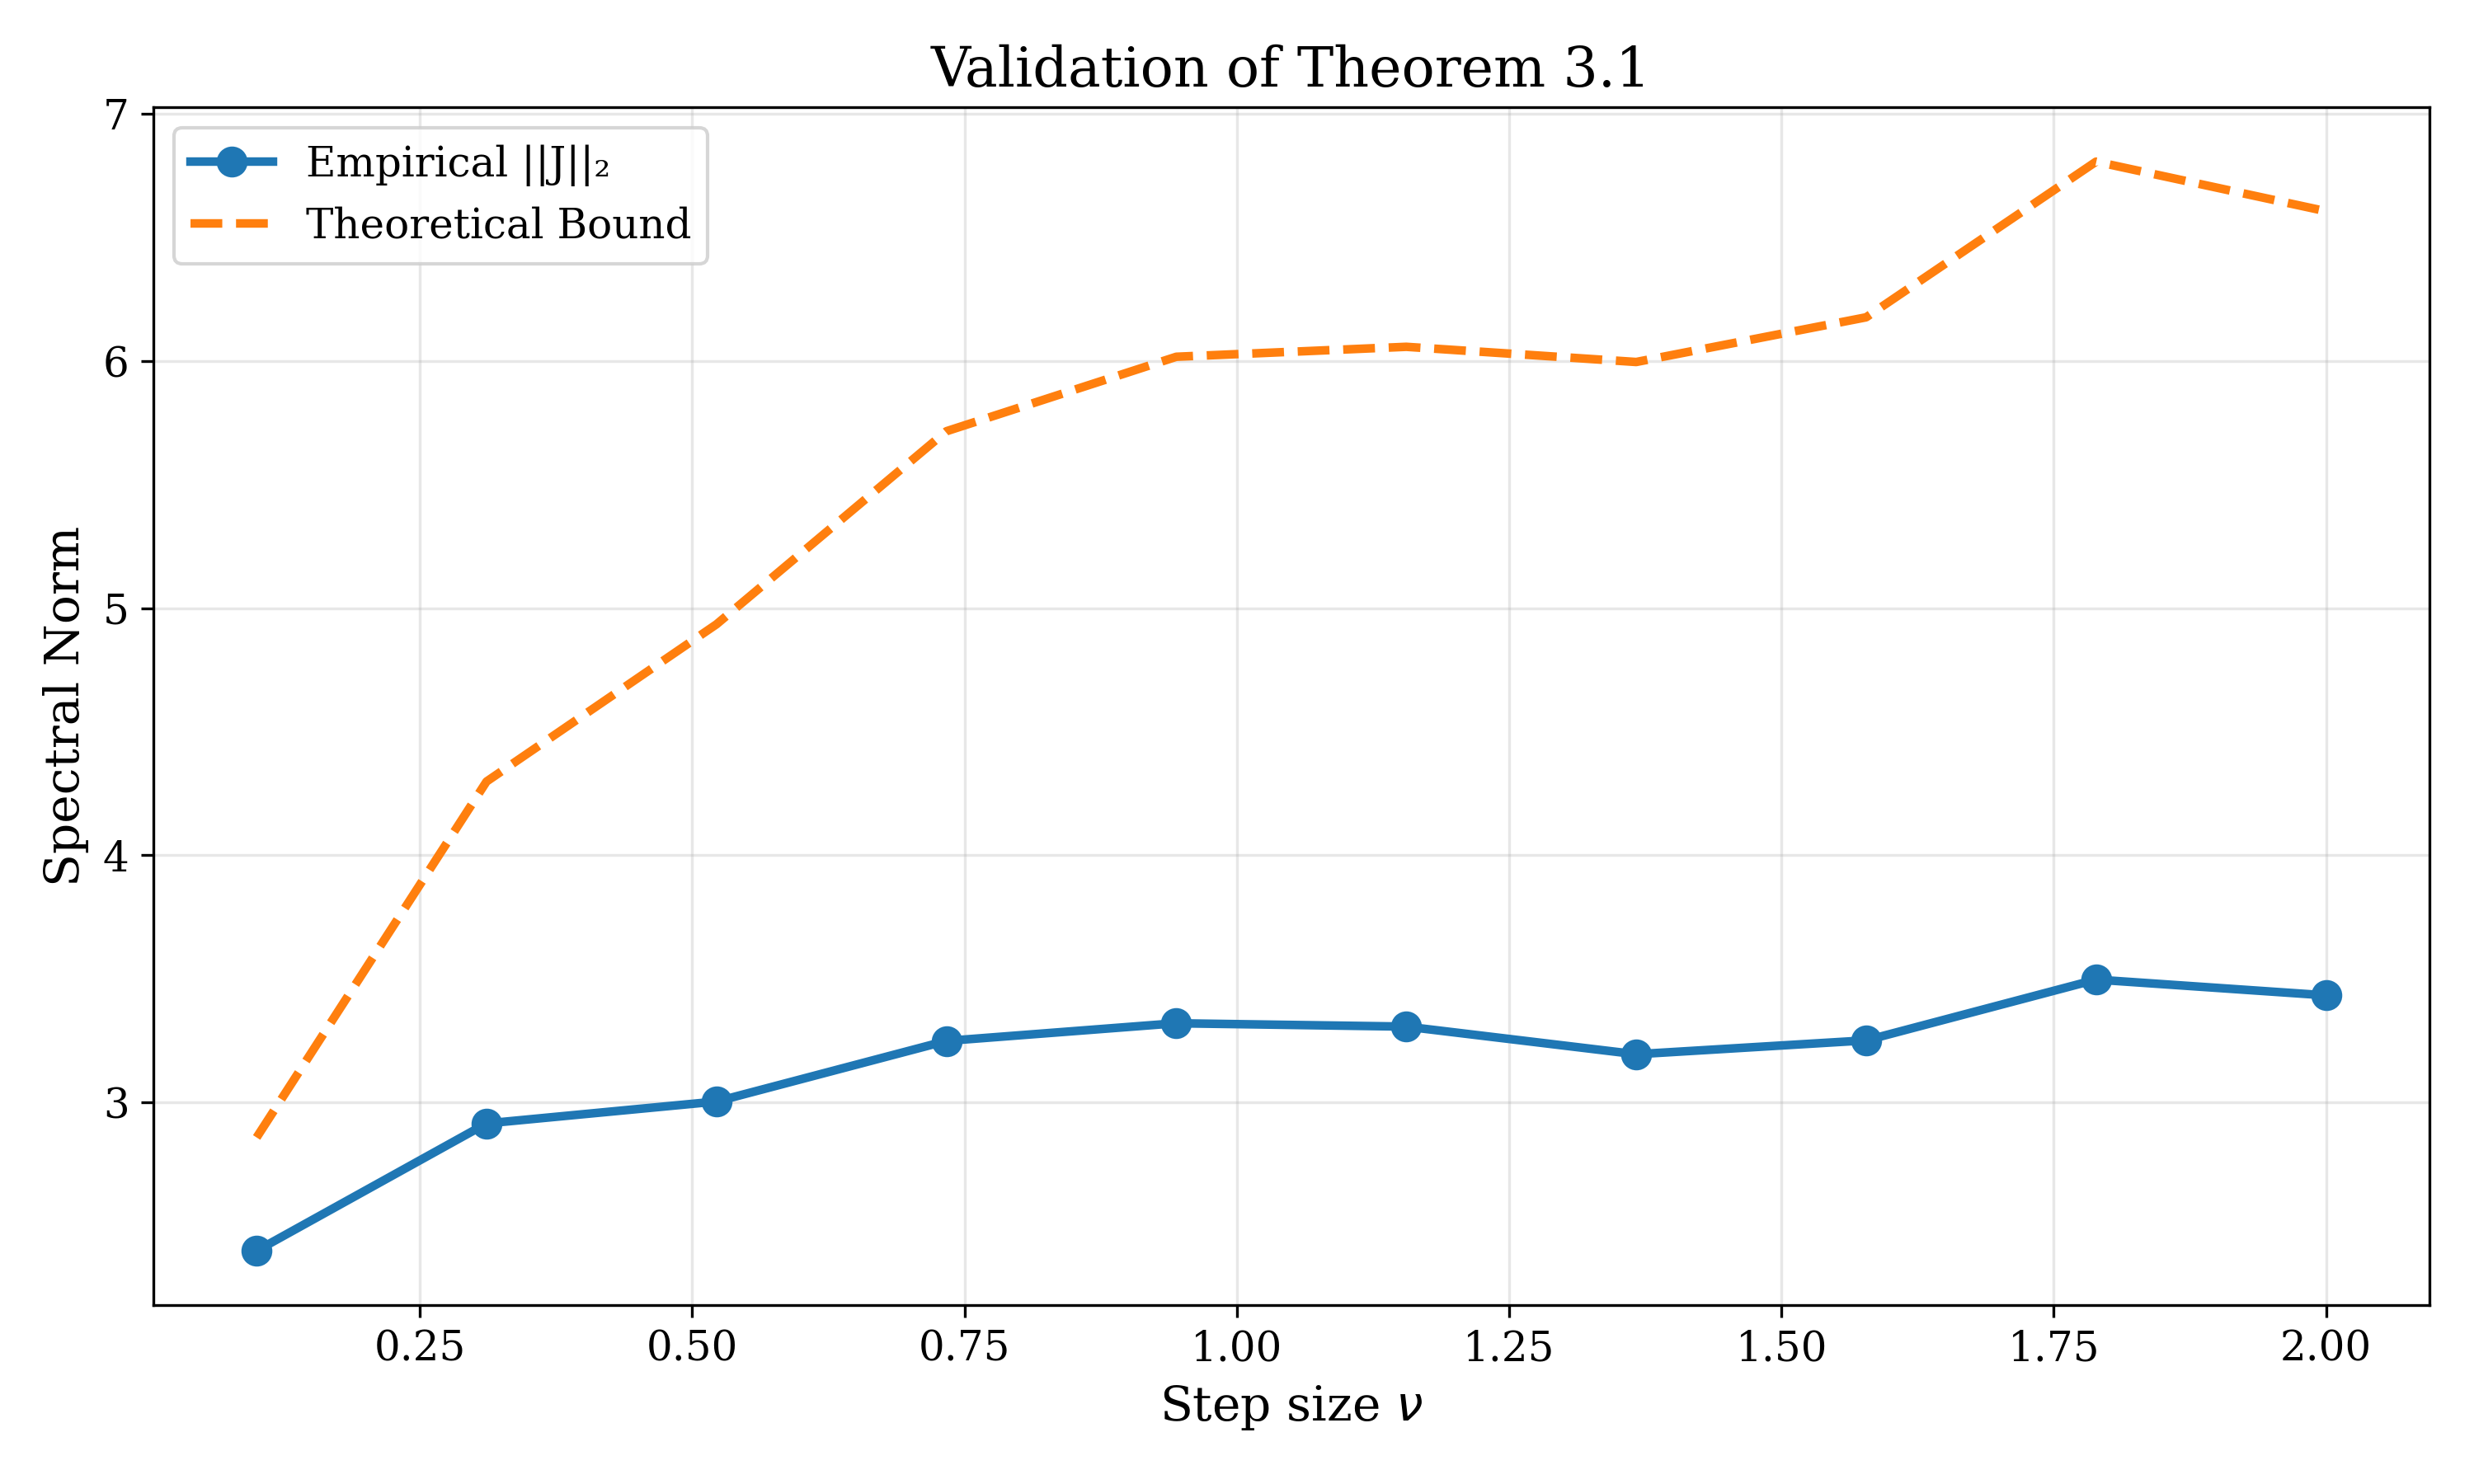
\includegraphics[width=0.73\textwidth]{old_plots_for_conference/fig1_bounds_validation.png}
        \caption{Empirical $\|J_F\|_2$ vs Theoretical Bound}
    \end{figure}
\end{frame}

% ---------------------------------------------------------------

\begin{frame}{Experiment 2: Validating Asymptotic Stability}
    \begin{figure}
        \centering
        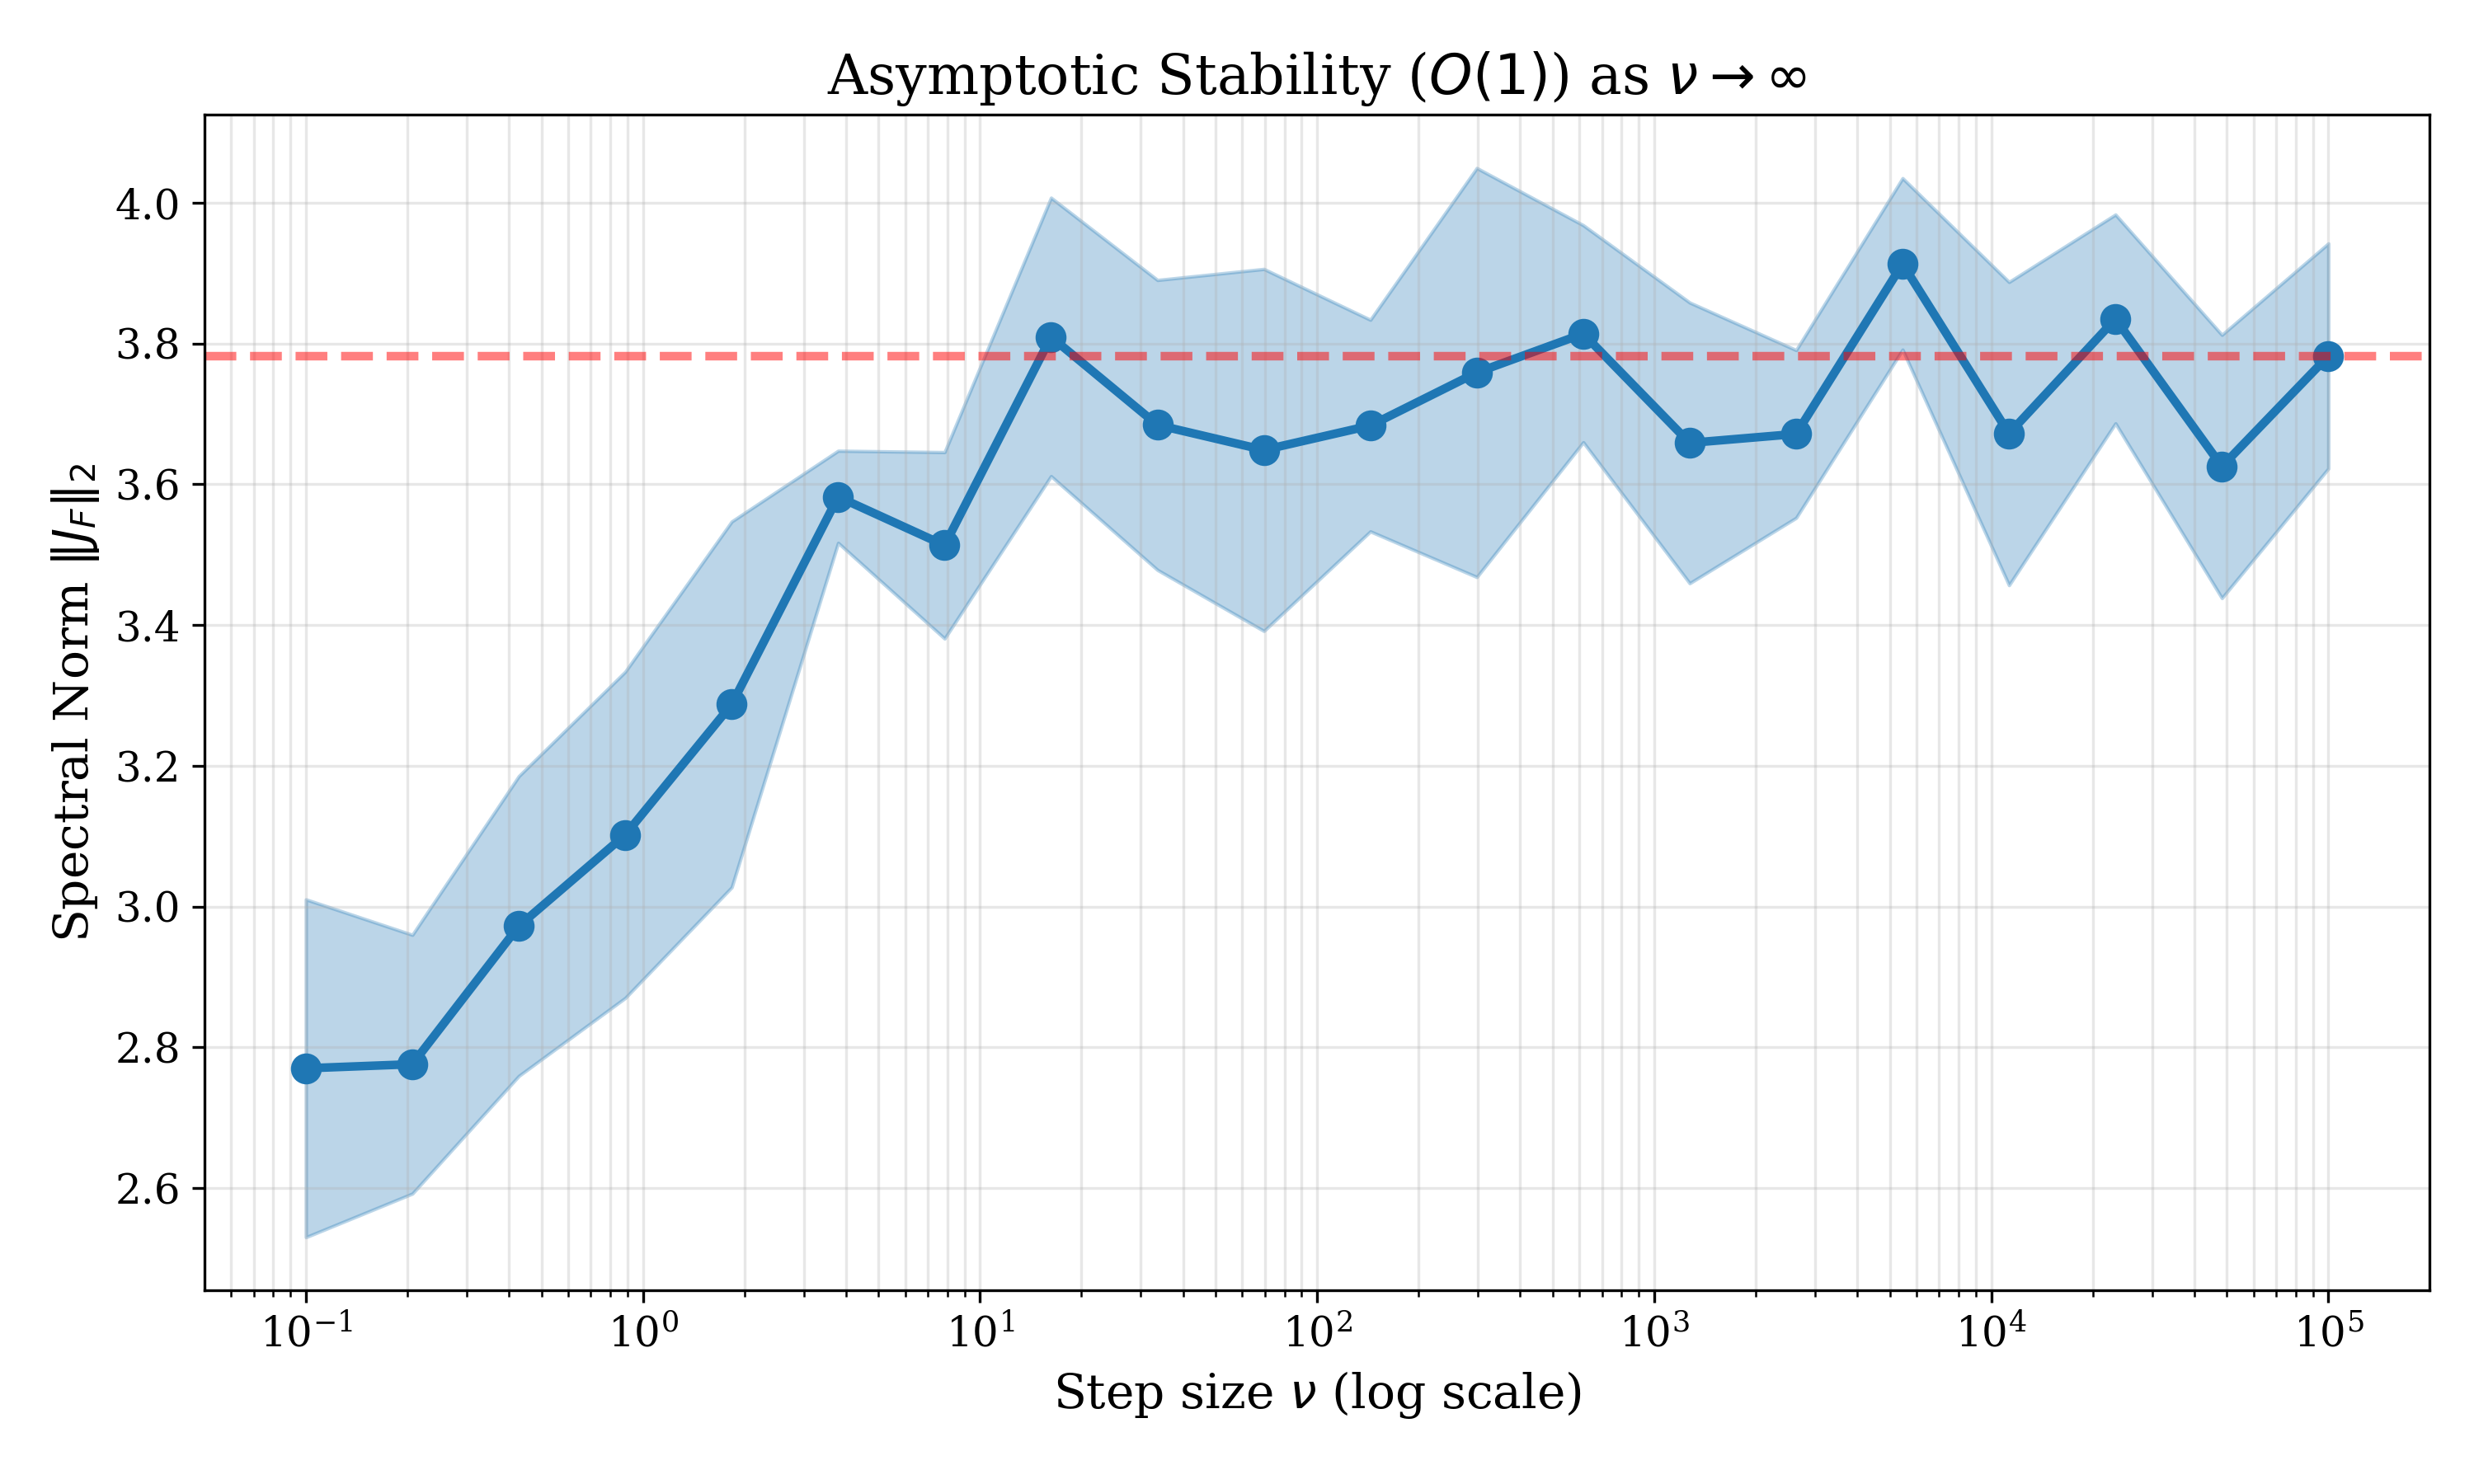
\includegraphics[width=0.73\textwidth]{old_plots_for_conference/fig2_asymptotic.png}
        \caption{Asymptotic Stability as $\nu \rightarrow \infty$}
    \end{figure}
\end{frame}

% ---------------------------------------------------------------
\begin{frame}{Experiment 3: Contraction on Embeddings}
    \begin{figure}
        \centering
        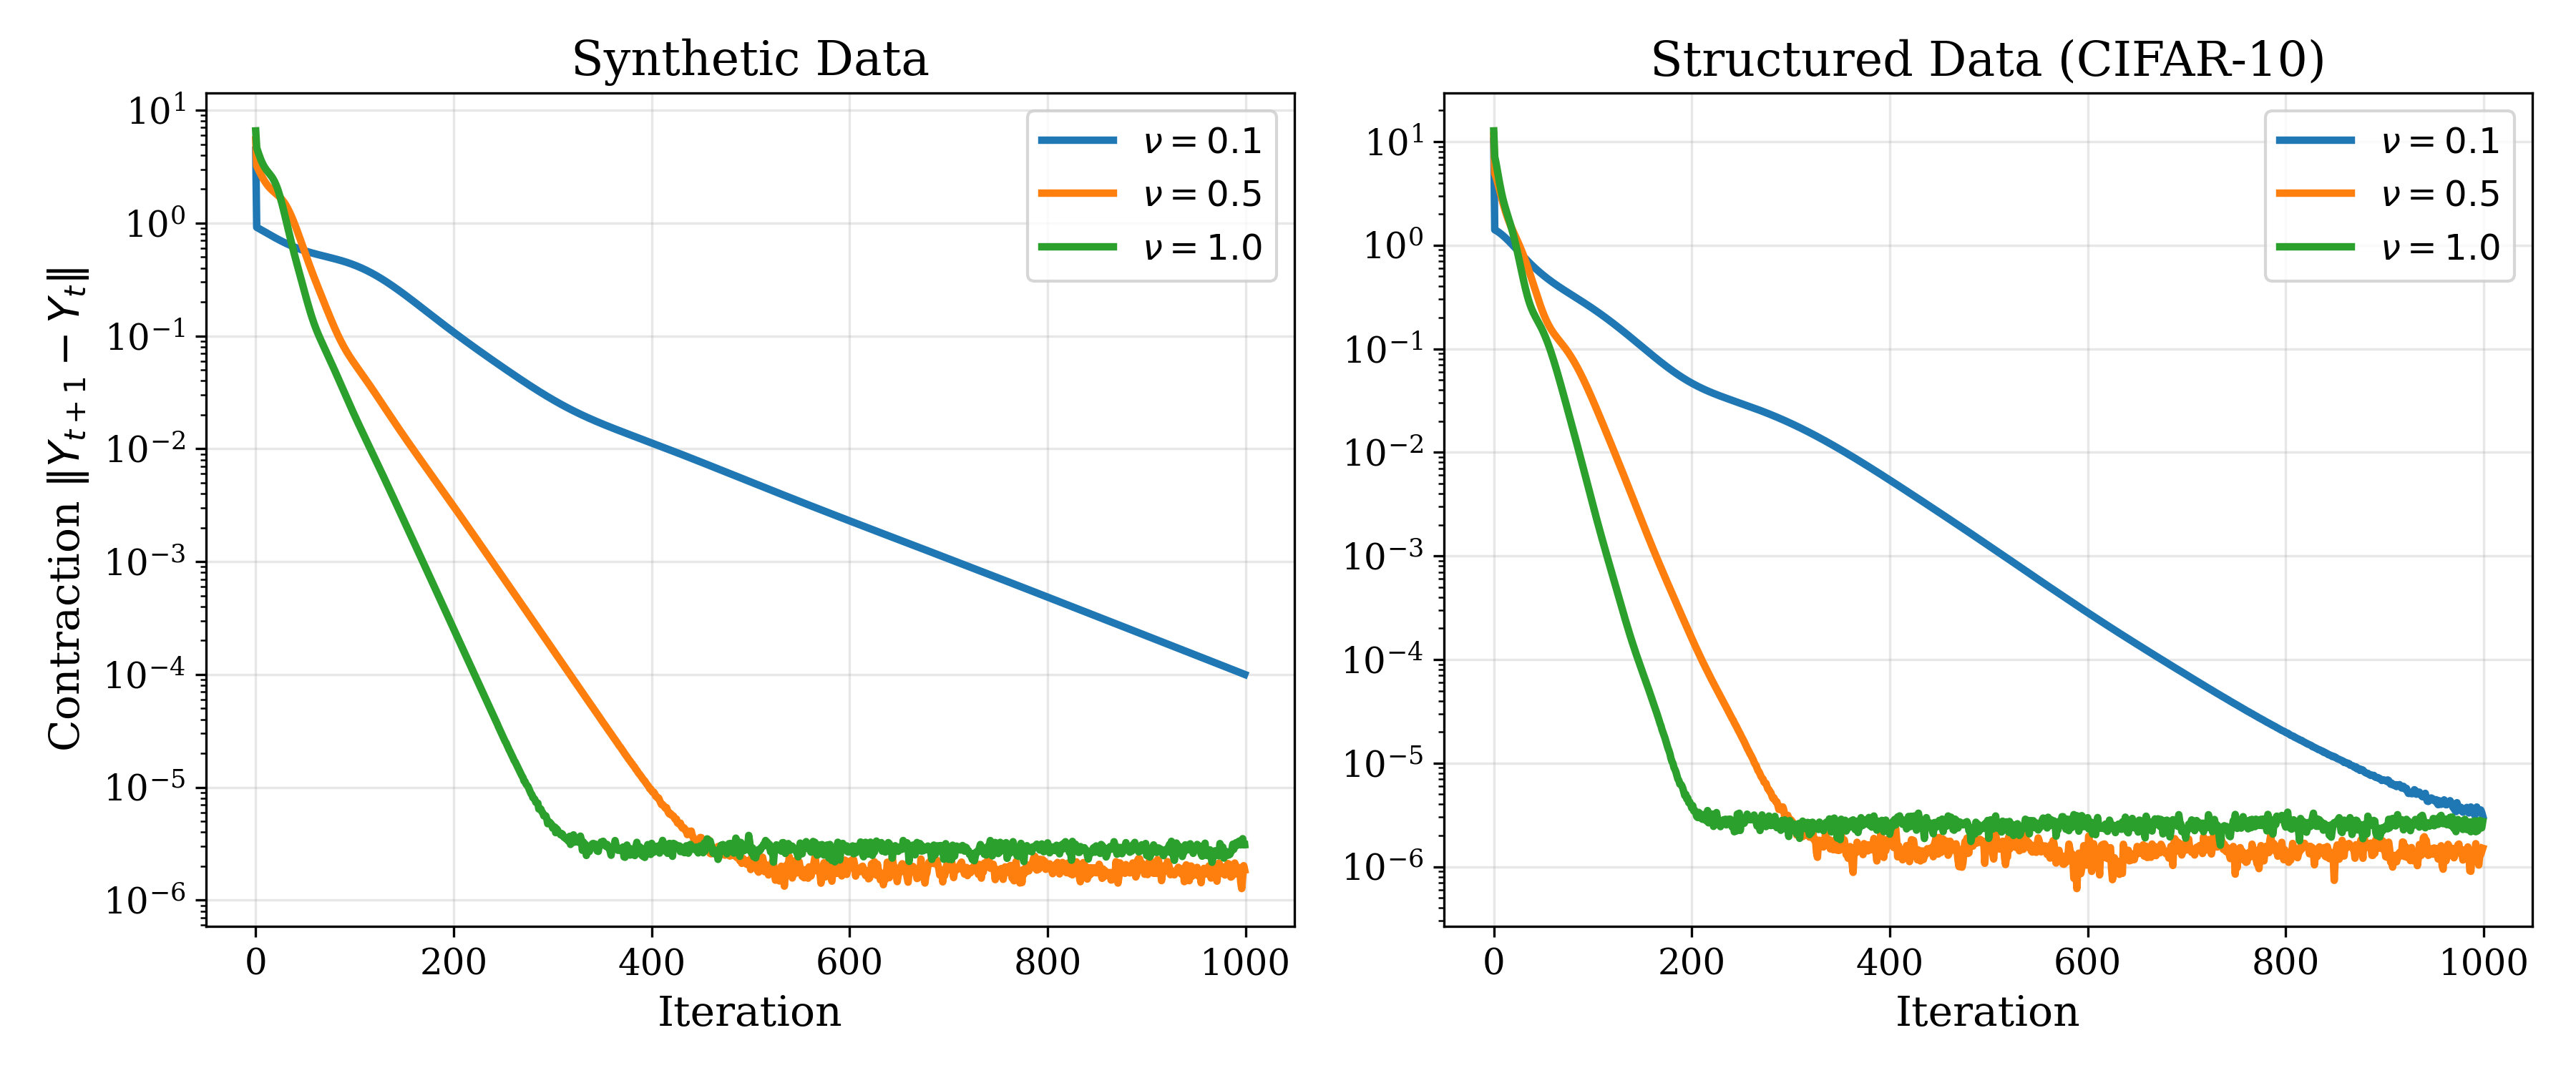
\includegraphics[width=1\textwidth]{old_plots_for_conference/fig3_contraction.png}
        \caption{Contraction dynamics on synthetic data and real embeddings.}
    \end{figure}
\end{frame}

% ---------------------------------------------------------------
\begin{frame}{Conclusion \& Future Work}
    \begin{columns}
        \begin{column}{0.5\textwidth}
            \textbf{Contributions:}
            \begin{itemize}
                \item Jacobian analysis of a full Transformer block.
                \item Explicit spectral bounds derived.
                \item Proved $O(1)$ stability for large $\nu$.
            \end{itemize}
        \end{column}
        \begin{column}{0.5\textwidth}
            \textbf{Future Directions:}
            \begin{itemize}
                \item Tightening the spectral bounds.
                \item Extension to Pre-Norm architectures.
                      % \item Link local Jacobian stability to global Deep Equilibrium limits.
            \end{itemize}
        \end{column}
    \end{columns}
\end{frame}

% ---------------------------------------------------------------
\begin{frame}[plain]
    \centering
    \vspace{3em}
    {\Huge \textcolor{miptblue}{\textbf{Thank you!}}}

    \vspace{2em}
    {\large \textbf{Paper, Slides \& Code:}} \\
    \vspace{0.5em}
    {\normalsize \href{https://github.com/Dimundel/Jacobian-Analysis-of-a-Recurrent-Transformer-Block}{Click here}}

    \vspace{2em}
    \small \textcolor{darkgray}{Dmitrii Vasilenko} \\
    \texttt{vasilenko.dmitrii@phystech.edu}
\end{frame}

\end{document}